% This is an example on how to add pictures to Latex. The first example will cover using an image as free floating position (i.e. The positioning of the image is decided on where it will fit with the least wastage of space)
% By convention all image files should be added to a separate image folder. It is just easier to organize the project files that way.
\section{An Example On How To Add Pictures}
Lorem ipsum dolor sit amet, consectetur adipiscing elit, sed do eiusmod tempor incididunt ut labore et dolore magna aliqua. Ut enim ad minim veniam, quis nostrud exercitation ullamco laboris nisi ut aliquip ex ea commodo consequat. Duis aute irure dolor in reprehenderit in voluptate velit esse cillum dolore eu fugiat nulla pariatur. Excepteur sint occaecat cupidatat non proident, sunt in culpa qui officia deserunt mollit anim id est laborum

Example of using a label to refer to a Figure \ref{fig:NodeMCU}

% Example of free floating image
\begin{figure}
    \centering
    % Playing around with the [width=.8] value will resize your image according to its width. It will scale appropriately. The name of the image file goes under the {NodeMCU}
    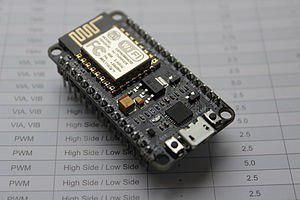
\includegraphics[width=.8\textwidth,center]{NodeMCU}
    \caption{NodeMCU Chip Diagram}
    % The label is useful when you want to refer to your image from text but you don't know what figure number it is.
    \label{fig:NodeMCU}
\end{figure}


\section{Fixed Image}Lorem ipsum dolor sit amet, consectetur adipiscing elit, sed do eiusmod tempor incididunt ut labore et dolore magna aliqua. Ut enim ad minim veniam, quis nostrud exercitation ullamco laboris nisi ut aliquip ex ea commodo consequat. Duis aute irure dolor in reprehenderit in voluptate velit esse cillum dolore eu fugiat nulla pariatur. Excepteur sint occaecat cupidatat non proident, sunt in culpa qui officia deserunt mollit anim id est laborum 

% To fix images to a certain section or sub section, do as follows

I want my image fixed here
 % The [H] after {figure} fixes the positioning of images.
\begin{figure}[H]
    \centering
    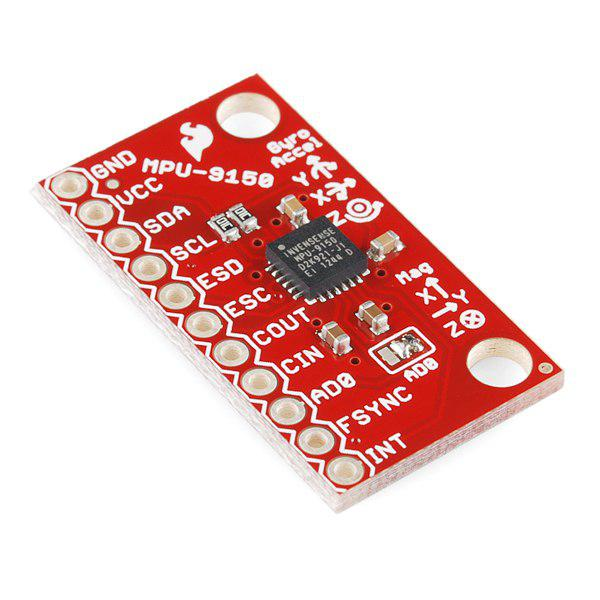
\includegraphics[width=.8\textwidth,center]{Inert}
    \caption{Inertial Measurement Unit}
    \label{fig:IMU}
\end{figure}

\section{Example on Table Usage}

Lorem ipsum dolor sit amet, consectetur adipiscing elit, sed do eiusmod tempor incididunt ut labore et dolore magna aliqua. Ut enim ad minim veniam, quis nostrud exercitation ullamco laboris nisi ut aliquip ex ea commodo consequat. Duis aute irure dolor in reprehenderit in voluptate velit esse cillum dolore eu fugiat nulla pariatur. Excepteur sint occaecat cupidatat non proident, sunt in culpa qui officia deserunt mollit anim id est laborum
\\
% To refer to the table use the same \ref{table:Spec}
To refer to the table use the same \ref{table:Spec}

\begin{table}[h!]
\centering
% To add another column in the table add another c in ||c c|| such that you get ||c c c|| for a three column table
\begin{tabular}{||c c||} 
 \hline
 %Every row entry is separated by a &. This is for Column titles.
 MPU 9150 Inertial Measurement Unit & NodeMCU Processor \\ [0.5ex] 
 \hline\hline
 % Data rows go here
 Acceleration Range: 2G & Dual-Core 80 Mhz Processor \\ 
 Gyroscope Range: 250 degrees/second  & 4MB Flash Memory \\
 Magnetometer Range: 1200 micro Teslas & 802.11 b/g/n connectivity \\
 Communication Protocol: I2C & \\[1ex] 
 \hline
\end{tabular}
\caption{Sensor Specifications}
\label{table:Spec}
\end{table}